% replace all text with your own text.
% in this template few examples are mention
\chapter{Methodology}
\label{ch:method} % Label for method chapter


\section{Data Collection}
Initially, the goal is to collect a large variety of information from many sources in order to have a thorough knowledge of the variables that lead to lung disease epidemics. Having access to both past and present information is made easier by partnerships with research groups, health departments, and healthcare organizations. Additionally, social media and internet-based sources of information complement traditional data streams, adding neighbourhood medical trends and public views of symptoms related to breathing to the dataset. A lung disease dataset is chosen from an online source Kaggle which contains the image of chest X-rays of 4 lung-related diseases. The model's input dataset is composed of multiple lung X-rays that have been gathered over time and labelled with four distinct breathing conditions. 
\subsection{Data Analysis}
\label{subsec:se_chpters}
A comprehensive analysis is performed on the gathered data to identify trends, patterns, and relationships related to lung disease epidemics. To learn more about the features of the dataset, initial investigation methods include data visualization, relationship matrices, and general statistics. Then, correlations between putative risk variables and the incidence of lung disease outbreaks are found using sophisticated statistical techniques including regression modelling and period analysis. Machine learning methods are used to find complicated relationships in the information, such as support vector machines and decision tree techniques. Preferences for choosing a model include understanding, adaptability, and reliability across various demographics and geographical areas. The accuracy and significance of data are improved for predictive modelling by data preparation. Enhancing the efficiency of models entails implementing features in addition to maintenance, normalizing, and assigning values that are not present. Overfitting hazards and computational difficulty are minimized through selected features and the reduction of dimensionality algorithms. Different test datasets are used in validation processes like bootstrapping to evaluate the efficiency and adaptability of the model. Compatibility with clinical standards and best practices is ensured by working alongside subject specialists.


\subsection{Data Processing}
Python simplifies interacting with data easier for users by providing a large number of built-in libraries for data processing and visualization. By highlighting trends and correlations, graphical representations of data, such as graphs and charts, make it easier to analyse and examine the data. Matplotlib and Seaborn are two popular Python libraries for data visualization that are available for usage in this context. These libraries include a variety of graphs that exhibit data in diverse ways, such as line plots, bar plots, and histograms. Density charts, for example, are useful for showing the shape of data and for calculating the probability density function and ongoing dataset allocation. By visualising data set descriptions and statistical distributions, box plots, on the other hand, are a useful tool for identifying possible outliers. 
\begin{figure}[ht]
    \centering
    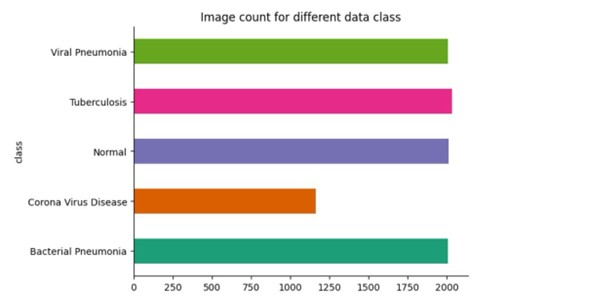
\includegraphics[scale=0.3]{figures/graph.jpg}
    \caption{Example figure in \LaTeX.}
    \label{fig:chart_a}
\end{figure}

Further processing the data, the dataset is split into 3 parts. 60 percent of the data is divided into training , 20 percent data is divided into validation and the remaining 20 percent of the data is divided into testing parts. This distributed dataset is passed on as input to train the models in a much more efficient and uniform manner. By splitting up the data set into training and testing sections, it is possible to train the model on the first one and assess its performance on the remaining part while the validation part will ensure the model’s accuracy on the trained data.In order for the model to train efficiently and produce precise predictions, this guarantees that the data is spread out accurately. Additionally, dividing the dataset prevents overfitting, a condition in which a model performs well on training data but badly on fresh data. 
\begin{figure}[ht]
    \centering
    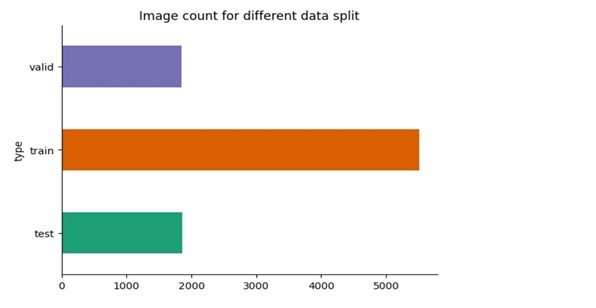
\includegraphics[scale=0.3]{figures/graph2.jpg}
    \caption{Example figure in \LaTeX.}
    \label{fig:chart_a}
\end{figure}


\subsection{Data Agumentation}
In order to increase the diversity of input data, data augmentation is used to add authentic yet unpredictable modifications to the training dataset that is supplied for neural network models. By minimally modifying the photos, it seeks to produce a copy of the original dataset. The method increases both the amount as well as the standard of the data. TensorFlow's Image Data Generator is used to apply different image-level alterations, such as height and width shifting, enlargement, and other required modifications, to the dataset. By making these little changes, the original dataset may be replicated with a greater degree of variability in the data. Rotation, width shift, zoom, and horizontal inversion are the four specific procedures that are used. The other changes are also done in this manner to make the dataset more diverse. In order to avoid underfitting and guarantee that the model gains knowledge from a variety of instances, image augmentation is especially applied to the training data.
\begin{figure}[ht]
    \centering
    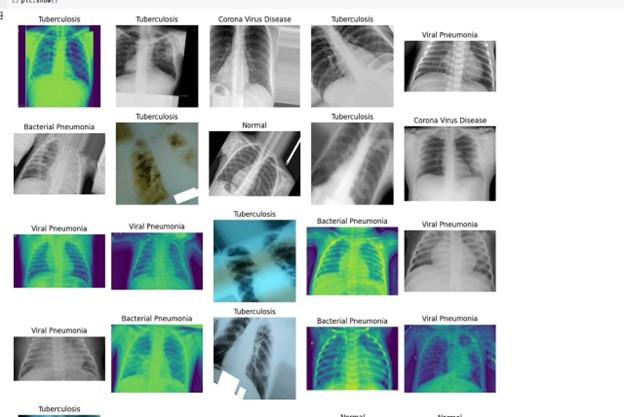
\includegraphics[scale=0.3]{figures/scan .jpg}
    \caption{Example figure in \LaTeX.}
    \label{fig:chart_a}
\end{figure}


\subsection{Example of a science lab-type main text structure}
If you are doing a science lab experiment type of project, you may use the  methodology section suggested in Table~\ref{tab:lab_temp}. In this kind of project, you may refer to the ``Methodology'' section as ``Materials and Methods.''


\section{Example of an Equation in \LaTeX}
Eq.~\ref{eq:eq_example} [note that this is an example of an equation's in-text citation] is an example of an equation in \LaTeX. In Eq.~\eqref{eq:eq_example}, $ s $ is the mean of elements $ x_i \in \mathbf{x} $: 

\begin{equation}
\label{eq:eq_example} % label used to refer the eq in text
s = \frac{1}{N} \sum_{i = 1}^{N} x_i. 
\end{equation}

Have you noticed that all the variables of the equation are defined using the \textbf{in-text} maths command \$.\$, and Eq.~\eqref{eq:eq_example} is treated as a part of the sentence with proper punctuation? Always treat an equation or expression as a part of the sentence. 

\section{Example of a Figure in \LaTeX}
Figure~\ref{fig:chart_a} is an example of a figure in \LaTeX. For more details, check the link:

\href{https://en.wikibooks.org/wiki/LaTeX/Floats,_Figures_and_Captions}{wikibooks.org/wiki/LaTeX/Floats,\_Figures\_and\_Captions}.

\noindent
Keep your artwork (graphics, figures, illustrations) clean and readable. At least 300dpi is a good resolution of a PNG format artwork. However, an SVG format artwork saved as a PDF will produce the best quality graphics. There are numerous tools out there that can produce vector graphics and let you save that as an SVG file and/or as a PDF file. One example of such a tool is the ``Flow algorithm software''. Here is the link for that: \href{http://www.flowgorithm.org/download/}{flowgorithm.org}.
\begin{figure}[ht]
    \centering
    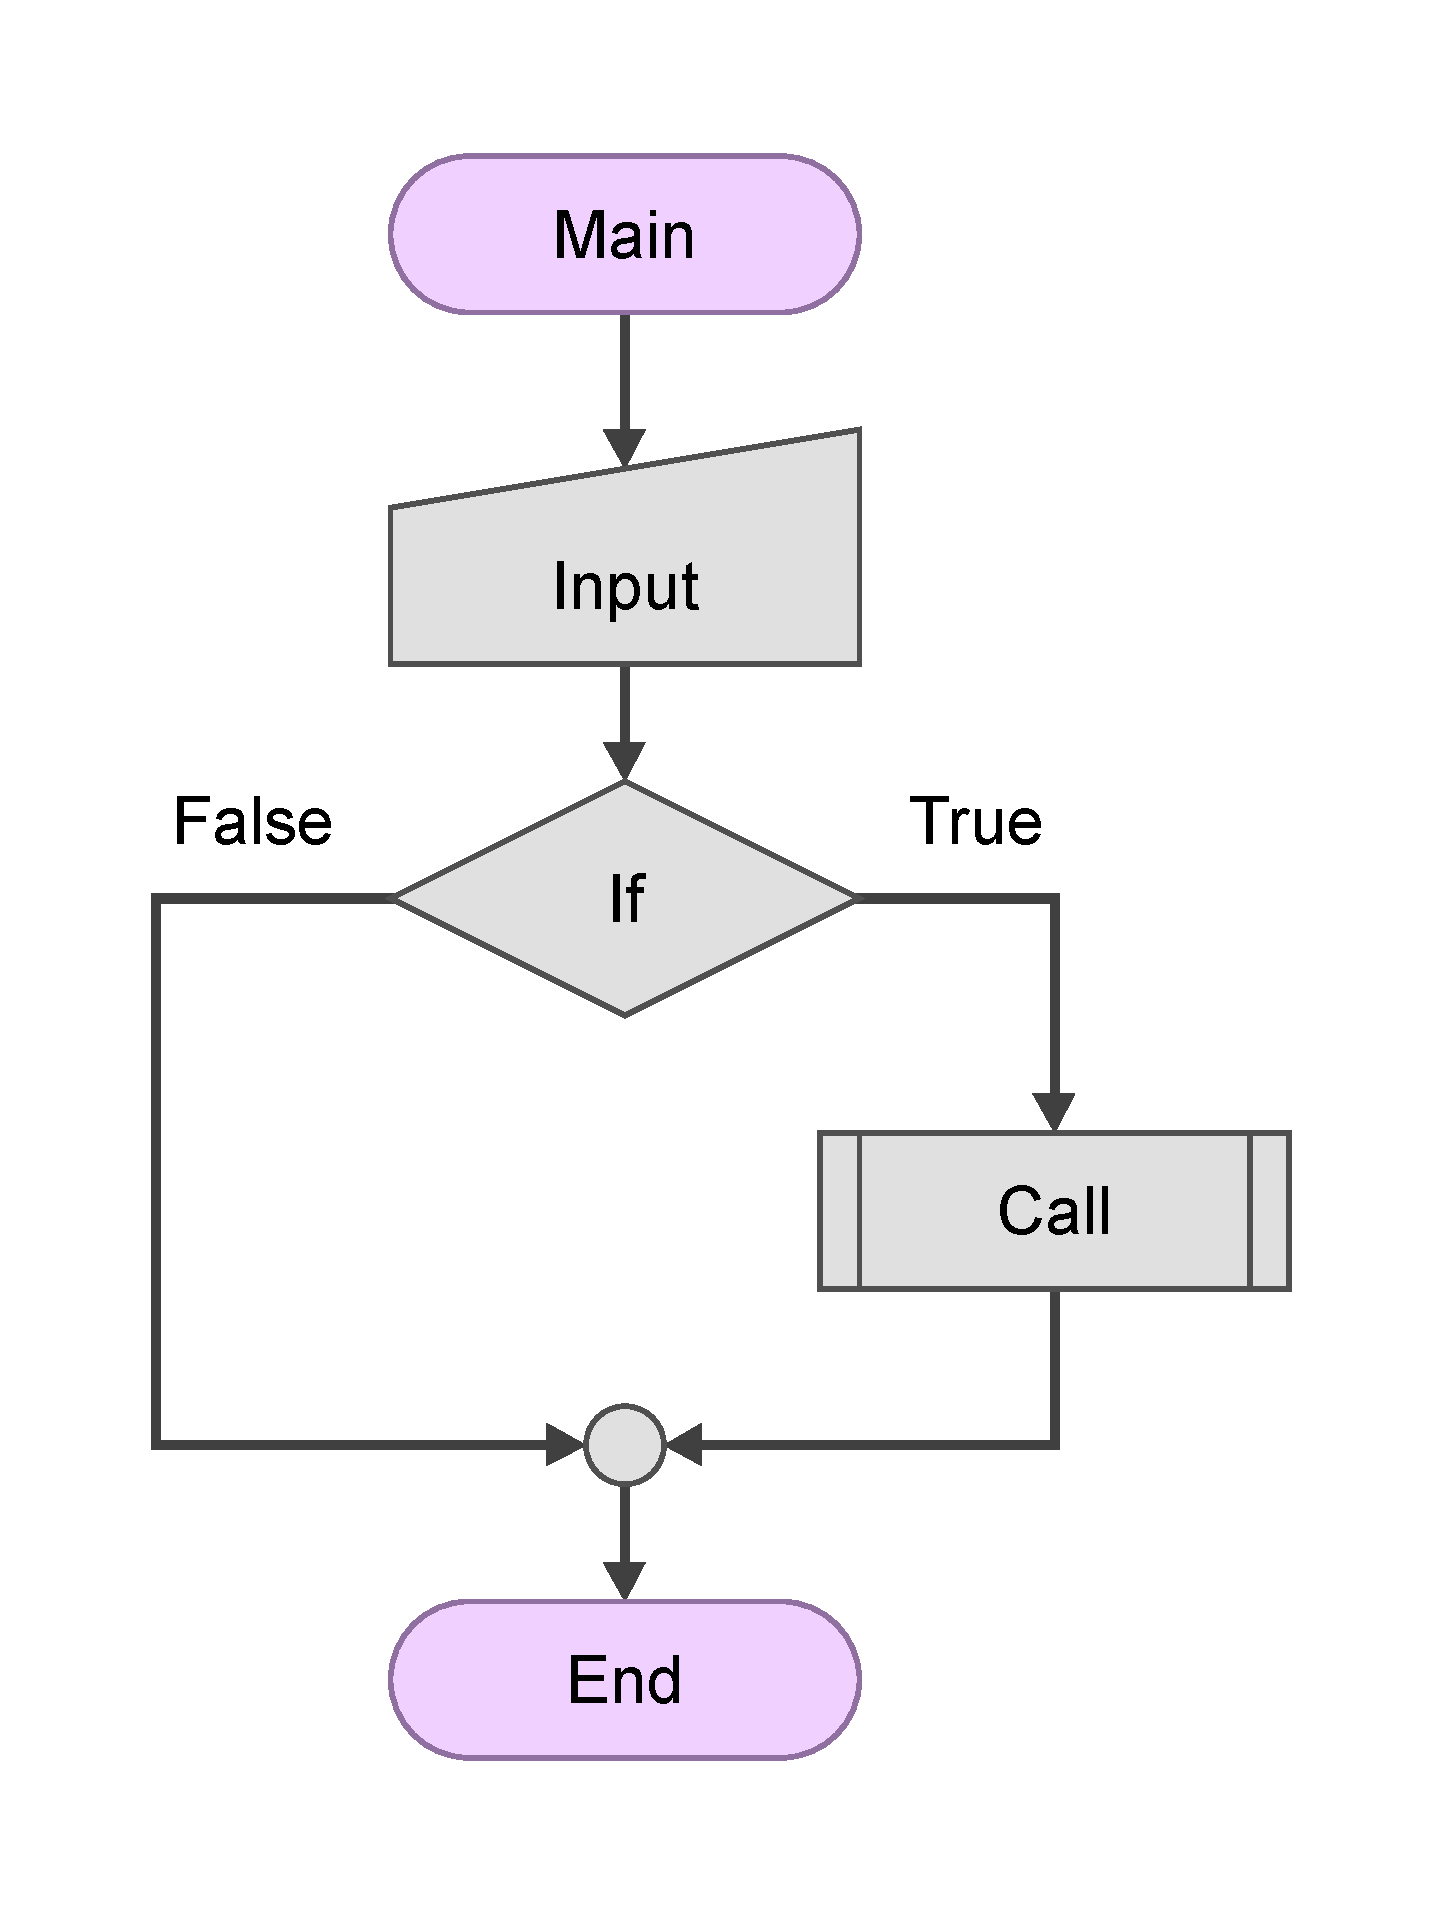
\includegraphics[scale=0.3]{figures/chart.pdf}
    \caption{Example figure in \LaTeX.}
    \label{fig:chart_a}
\end{figure}

\clearpage %  use command \clearpage when you want section or text to appear in the next page.

\section{Example of an algorithm in \LaTeX}
Algorithm~\ref{algo:algo_example} is a good example of an algorithm in \LaTeX.  
\begin{algorithm}
    \caption{Example caption: sum of all even numbers}
    \label{algo:algo_example}
    \begin{algorithmic}[1]
        \Require{$ \mathbf{x}  = x_1, x_2, \ldots, x_N$}
        \Ensure{$EvenSum$ (Sum of even numbers in $ \mathbf{x} $)}
        \Statex
        \Function{EvenSummation}{$\mathbf{x}$}
        \State {$EvenSum$ $\gets$ {$0$}}
        \State {$N$ $\gets$ {$length(\mathbf{x})$}}
        \For{$i \gets 1$ to $N$}                    
        \If{$ x_i\mod 2 == 0$}  \Comment check if a number is even?
        \State {$EvenSum$ $\gets$ {$EvenSum + x_i$}}
        \EndIf
        \EndFor
        \State \Return {$EvenSum$}
        \EndFunction
    \end{algorithmic}
\end{algorithm}
 
\section{Example of code snippet  in \LaTeX}

Code Listing~\ref{list:python_code_ex} is a good example of including a code snippet in a report. While using code snippets, take care of the following:
\begin{itemize}
    \item do not paste your entire code (implementation) or everything you have coded. Add code snippets only. 
    \item The algorithm shown in Algorithm~\ref{algo:algo_example} is usually preferred over code snippets in a technical/scientific report. 
    \item Make sure the entire code snippet or algorithm stays on a single page and does not overflow to another page(s).  
\end{itemize}

Here are three examples of code snippets for three different languages (Python, Java, and CPP) illustrated in Listings~\ref{list:python_code_ex}, \ref{list:java_code_ex}, and \ref{list:cpp_code_ex} respectively.  

\begin{lstlisting}[language=Python, caption={Code snippet in \LaTeX ~and  this is a Python code example}, label=list:python_code_ex]
import numpy as np

x  = [0, 1, 2, 3, 4, 5] # assign values to an array
evenSum = evenSummation(x) # call a function

def evenSummation(x):
    evenSum = 0
    n = len(x)
    for i in range(n):
        if np.mod(x[i],2) == 0: # check if a number is even?
            evenSum = evenSum + x[i]
    return evenSum
\end{lstlisting}

Here we used  the ``\textbackslash clearpage'' command and forced-out the second listing example onto the next page. 
\clearpage  %
\begin{lstlisting}[language=Java, caption={Code snippet in \LaTeX ~and  this is a Java code example}, label=list:java_code_ex]
public class EvenSum{ 
    public static int evenSummation(int[] x){
        int evenSum = 0;
        int n = x.length;
        for(int i = 0; i < n; i++){
            if(x[i]%2 == 0){ // check if a number is even?
                evenSum = evenSum + x[i];
            }
        }
        return evenSum;     
    }
    public static void main(String[] args){ 
        int[] x  = {0, 1, 2, 3, 4, 5}; // assign values to an array
        int evenSum = evenSummation(x);
        System.out.println(evenSum);
    } 
} 
\end{lstlisting}


\begin{lstlisting}[language=C, caption={Code snippet in \LaTeX ~and  this is a C/C++ code example}, label=list:cpp_code_ex]
int evenSummation(int x[]){
    int evenSum = 0;
    int n = sizeof(x);
    for(int i = 0; i < n; i++){
        if(x[i]%2 == 0){ // check if a number is even?
            evenSum = evenSum + x[i];
    	}
    }
    return evenSum;     
}

int main(){
    int x[]  = {0, 1, 2, 3, 4, 5}; // assign values to an array
    int evenSum = evenSummation(x);
    cout<<evenSum;
    return 0;
}
\end{lstlisting}



\section{Example of in-text citation style}
\subsection{Example of the equations and illustrations placement and reference in the text}
Make sure whenever you refer to the equations, tables, figures, algorithms,  and listings for the first time, they also appear (placed) somewhere on the same page or in the following page(s). Always make sure to refer to the equations, tables and figures used in the report. Do not leave them without an \textbf{in-text citation}. You can refer to equations, tables and figures more them once.

\subsection{Example of the equations and illustrations style}
Write \textbf{Eq.} with an uppercase ``Eq`` for an equation before using an equation number with (\textbackslash eqref\{.\}). Use ``Table'' to refer to a table, ``Figure'' to refer to a figure, ``Algorithm'' to refer to an algorithm and ``Listing'' to refer to listings (code snippets). Note that, we do not use the articles ``a,'' ``an,'' and ``the'' before the words Eq., Figure, Table, and Listing, but you may use an article for referring the words figure, table, etc. in general.

For example, the sentence ``A report structure is shown in \textbf{the} Table~\ref{tab:gen_template}'' should be written as ``A report structure is shown \textbf{in} Table~\ref{tab:gen_template}.'' 
 

\section{Summary}
Write a summary of this chapter.

~\\[5em]
\noindent
{\huge\textbf{Note:}} In the case of \textbf{software engineering} project a Chapter ``\textbf{Testing and Validation}'' should precede the ``Results'' chapter. See Section~\ref{subsec:se_chpters} for report organization of such project. 

